\documentclass[11pt]{amsart}


\usepackage{geometry}                % See geometry.pdf to learn the layout options. There are lots.
\geometry{a4paper}                   % ... or a4paper or a5paper or ...
%\geometry{landscape}                % Activate for for rotated page geometry
\usepackage[parfill]{parskip}    % Activate to begin paragraphs with an empty line rather than an indent
\usepackage{enumitem}
\usepackage{graphicx}
\usepackage{amssymb}
\usepackage{amsmath}
\usepackage{cancel}
\usepackage{epstopdf}
\DeclareGraphicsRule{.tif}{png}{.png}{`convert #1 `dirname #1`/`basename #1 .tif`.png}
\usepackage{breqn}
\usepackage{float}

\title{Econ 210C Problem Set \# 3}
\author{Minki Kim}
%\date{}                                           % Activate to display a given date or no date

\begin{document}




\maketitle

\section{Variable labor supply in the RBC model}
\begin{figure}[H]
	\centering
	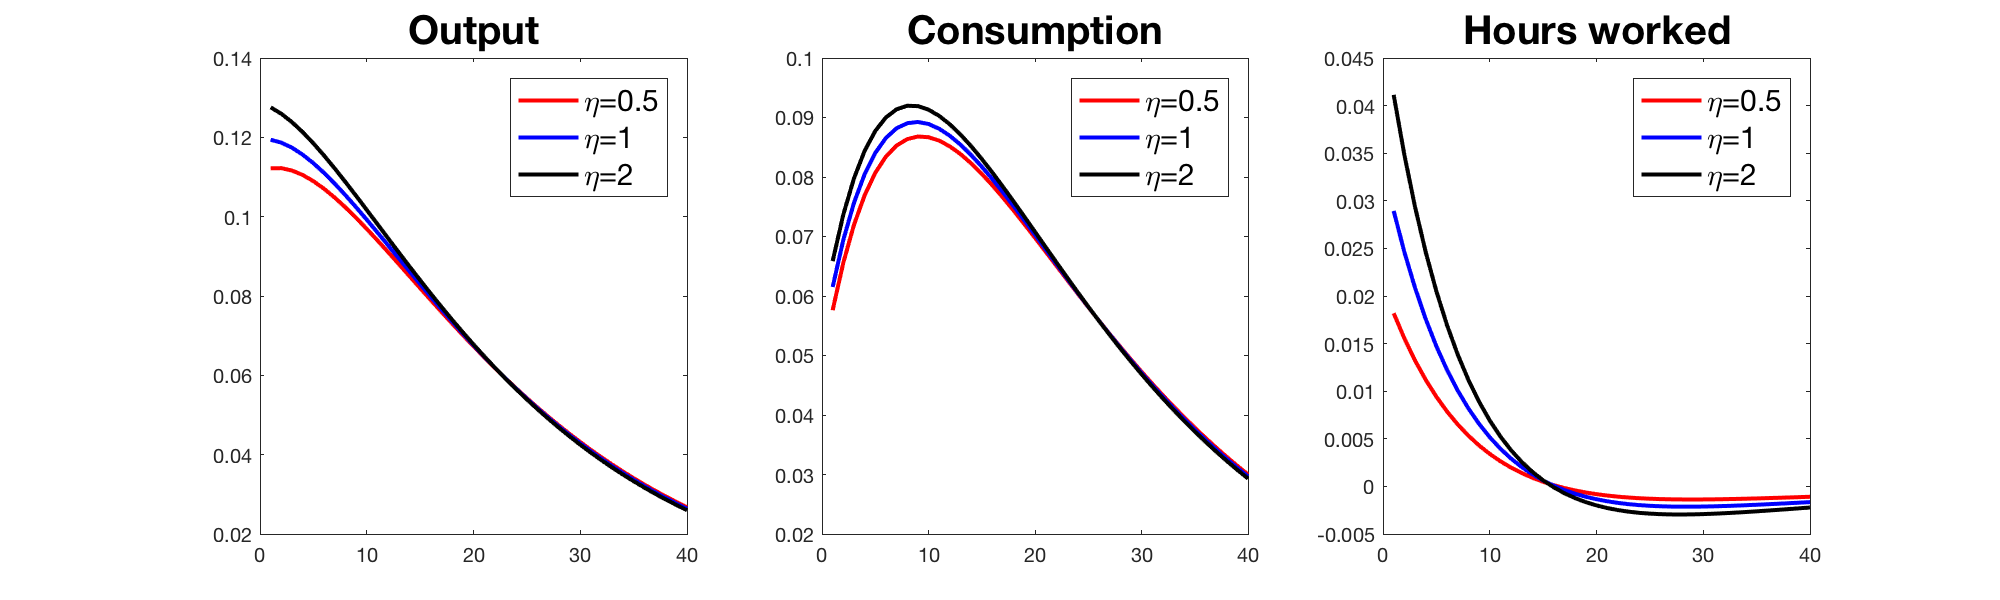
\includegraphics[width=\textwidth]{Q1}
	\caption{Impulse responses with varying $\eta$}
\end{figure}

\begin{table}[H]
	\centering
	\begin{tabular}{ccccc}
		\hline \hline 
		& $\eta=0.5$  & $\eta = 1$          & $\eta = 2$ & Data  \\
		\hline 
		$Stdev(Y)$ &  1.54    & 1.64    & 1.74    & 1.72     \\
		$Stdev(C)$ &  0.97    & 1.02   & 1.08       & 1.27 \\
		$Stdev(L)$ &   0.23   &  0.37   & 0.53     &  1.59 \\
		\hline
	\end{tabular}
	\caption{Response to a transitory discount factor shock}
\end{table}
As one would expect, the fits get better as we calibrate the Frisch elasticity to bigger values. A large Frisch elasticity generates stronger intertemporal substitution of labor suppply, and hence amplifies the effect of shocks. However, even with a large Frisch elasticity, consumption is too smooth, and the volatility of hours generated from the model falls short of the empirical counterpart. 




\end{document}
